\documentclass[compress]{beamer}
\mode<presentation>

\usetheme{Warsaw}
\definecolor{innotek}{RGB}{2,52,173}
\setbeamercolor*{palette primary}{use=structure,fg=white,bg=innotek}
%\usecolortheme[RGB={2,52,173}]{structure}
\defbeamertemplate*{footline}{shadow theme}
{%
  \leavevmode%
  \hbox{\begin{beamercolorbox}[wd=.5\paperwidth,ht=2.5ex,dp=1.125ex,leftskip=.3cm plus1fil,rightskip=.3cm]{author in head/foot}%
    \usebeamerfont{author in head/foot}\hfill\insertshortauthor%
  \end{beamercolorbox}%
  \begin{beamercolorbox}[wd=.5\paperwidth,ht=2.5ex,dp=1.125ex,leftskip=.3cm,rightskip=.3cm plus1fil]{title in head/foot}%
      \usebeamerfont{title in head/foot}\insertshorttitle\hfill\insertframenumber\,/\,\inserttotalframenumber%
  \end{beamercolorbox}}%
  \vskip0pt%
}
\setbeamertemplate{navigation symbols}{}%remove navigation symbols

\usepackage{subfigure}
\usepackage{multicol}
\usepackage{amsmath}
\usepackage{epsfig}
\usepackage{graphicx}
\usepackage[all,knot]{xy}
\xyoption{arc}
\usepackage{url}
\usepackage{multimedia}
\usepackage{hyperref}
\usepackage{setspace}

\usepackage{lmodern}% http://ctan.org/pkg/lm

% define your own colours:
\definecolor{innotek}{RGB}{1,54,160}
\definecolor{Red}{rgb}{1,0,0}
\definecolor{Blue}{rgb}{0,0,1}
\definecolor{Green}{rgb}{0,1,0}
\definecolor{magenta}{rgb}{1,0,.6}
\definecolor{lightblue}{rgb}{0,.5,1}
\definecolor{lightpurple}{rgb}{.6,.4,1}
\definecolor{gold}{rgb}{.6,.5,0}
\definecolor{orange}{rgb}{1,0.4,0}
\definecolor{hotpink}{rgb}{1,0,0.5}
\definecolor{newcolor2}{rgb}{.5,.3,.5}
\definecolor{newcolor}{rgb}{0,.3,1}
\definecolor{newcolor3}{rgb}{1,0,.35}
\definecolor{darkgreen1}{rgb}{0, .35, 0}
\definecolor{darkgreen}{rgb}{0, .6, 0}
\definecolor{darkred}{rgb}{.75,0,0}

\xdefinecolor{olive}{cmyk}{0.64,0,0.95,0.4}
\xdefinecolor{purpleish}{cmyk}{0.75,0.75,0,0}

\useoutertheme[subsection=false]{smoothbars}

\title{DRINC}
\subtitle{Dynamically Refreshing Interplexing Number of Cordials}
\author[]{Brandon Arnold\\Hoang Phan\\Owen Ledvina\\Kyle Timins}
\date{December $6^{th}$, 2013}


\AtBeginSection[]
{
  \begin{frame}
    \frametitle{Table of Contents}
    \tableofcontents[currentsection,hideallsubsections]
  \end{frame}
}

\begin{document}

\frame{
    \titlepage
}

\begin{frame}
\frametitle{Table of Contents}
\tableofcontents[hideallsubsections]
\end{frame}

\section*{Introduction}
\frame{
 \frametitle{Introduction}
    \begin{itemize}
        \item What is DRINC?
        \item Interfaces
        \item Server
        \item Pouring Device
    \end{itemize}
}


\section{Functional Requirements}
\subsection{Hardware}

\begin{frame}
    \frametitle{Hareware Requirements}
    \begin{itemize}
        \item {\large Frame: Must hold:}
        \begin{itemize}
            \item 9 liter sized glass bottles, control system, transport track
        \end{itemize}
        \item {\large Power Supply:}
        \begin{itemize}
            \item Be able to power all systems in the DRINC
        \end{itemize}
        \item {\large Back End Control Systems:}
        \begin{itemize}
            \item Be able to control all mixing hardware with one micro 
            processor
            \item Be able to run main system on one microprocessor and interact 
            with other microprocessor
        \end{itemize}
    \end{itemize}
\end{frame}

\begin{frame}
    \frametitle{Hardware Requirements Cont.}
    \begin{itemize}
        \item {\large Drink Transport Track:}
        \begin{itemize}
            \item Transport cups safely, securely, and accurately on a square 
            grid
        \end{itemize}
        \item {\large Track Servos:}
        \begin{itemize}
            \item Two servos strong enough to move a full pint of liquid and 
            glass reliably
        \end{itemize}
        \item {\large Valves:}
        \begin{itemize}
            \item Installed on each bottle
            \item Ability to turn on and off quickly by backend system to pour ~
            40ml parts
        \end{itemize}
    \end{itemize}
\end{frame}

\subsection{Software}

\begin{frame}
    \frametitle{Software Requirements}
    \begin{itemize}
        \item {\large Website:}
        \begin{itemize}
            \item Log on and off authentication using backend database
            \item After successful authentication, user is presented with a menu:
            \begin{itemize}
                \item Create a Custom Drink
                \item Select a Drink
                \item Most Drank
                \item Delete a Drink
            \end{itemize}
        \end{itemize}
    \end{itemize}
\end{frame}

\begin{frame}
    \frametitle{Software Requirements Cont.}
    \begin{itemize}
        \item {\large Backend Server:}
        \begin{itemize}
            \item Hold drink information and send to DRINC
            \item Ability to SSH into machine for maintenance or configuration
            \item Keep track of the drinks consumed by the user during time period
        \end{itemize}
    \end{itemize}
\end{frame}




\section{Non-Function Requirements}
\chapter{Nonfunctional Requirements}

{
    \renewcommand*{\theenumi}{\thesubsection.\arabic{enumi}}
    \renewcommand*{\theenumii}{\theenumi.\arabic{enumii}}
    \renewcommand*{\theenumiii}{\theenumii.\arabic{enumiii}}
    
    \section{Hardware Considerations}
	Most hardware should emphasize low cost.    
    
    \subsection{Valves}
    Valves should be made of plastic or a non copper or copper alloy metal so as not to kill the user via copper poisoning.
	\subsection{Frame}
    Frame should be modular and easily disassemble for transportation.

 	\section{User Interface}
 	
 	\subsection{Website}
 	\begin{enumerate}
    	\item Shall allow the user to do any task in the least amount of click/push/touch
   	 	\item The site should look visually appealing, with lack of ``clutter''
    	\item The website will be written in html and php
    	\item The website database will be managed with postgreSQL
    	\item The ingredient list and amount list will be created using HTML <select> tag
    	\item When a drink is labeled as ``Selected'', it will be highlighted using Javascript
    \end{enumerate}
    \subsection{Android App}
    \begin{enumerate}
    	\item The Android app should look very similar to the website.
   		\item Allow the user to log in via a wireless technology\
   	\end{enumerate}
	\subsection{Backend Server}
	\begin{enumerate}
		\item Any updates must be started on Wednesday after 10:00AM and finish before 12:00PM.
		\item The server must handle all login and logout requests in under 200ms.
   		\item Ability to add a drink recipe with ease
	\end{enumerate}
    
    }
    




\section{Interfaces}
\begin{frame}
    \frametitle{Interfaces}
    \begin{itemize}
        \item {\large Web Site:}
        \begin{itemize}
            \item Should all the user to do any task in the least amount of 
            clicks
            \item Should look visually appealign, with lack of ``clutter''
        \end{itemize}
        \item {\large Android Device:}
        \begin{itemize}
            \item Follow same UI and visual requirements as the website
            \item Will allow the user to log in via a wireless technology
        \end{itemize}
    \end{itemize}
\end{frame}

\subsection{Website}
\begin{frame}
    \frametitle{Website}
    \begin{itemize}
        \item Django/Python, HTML, CSS, Javascript
        \item PostgreSQL
        \item Administrative functions
    \end{itemize}
\end{frame}

\subsection{Android Device}
\begin{frame}
    \frametitle{Android Device}
    \begin{itemize}
        \item {\large Nexus 7}
        \begin{itemize}
            \item App will be build in the Android version of Java and XML
            \item Device will be attached to the DRINC machine
        \end{itemize}
    \end{itemize}
\end{frame}

\begin{frame}
    \frametitle{Android Mock-up}
    \begin{figure}[htb]
        \centering
        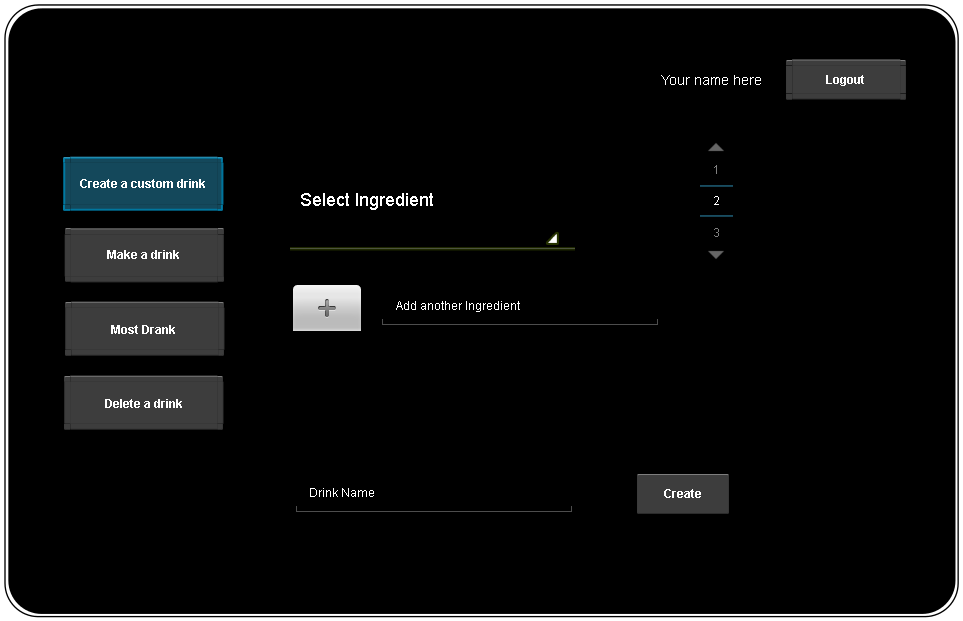
\includegraphics[width=0.8\textwidth]{../Mock-ups/Android_CreateDrink.png}
        \caption{Example of creating a drink on the Android device}
        \label{fig:CreateDrinkAndroid}
    \end{figure}
\end{frame}
\begin{frame}
    \frametitle{Android Mock-up}
    \begin{figure}[htb]
        \centering
        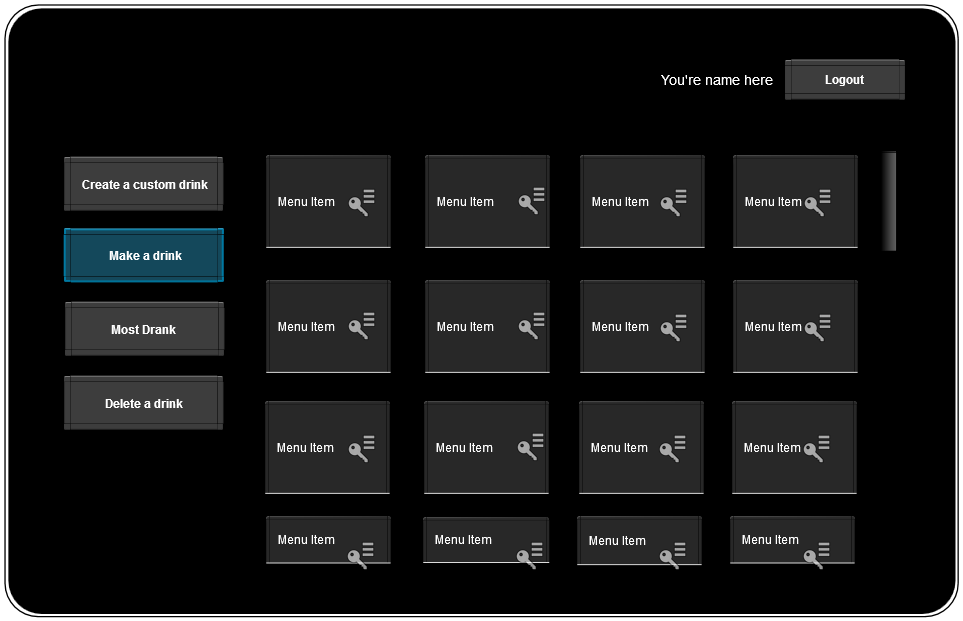
\includegraphics[width=0.8\textwidth]{../Mock-ups/Android_SelectDrink.png}
        \caption{Example of selecting a drink on the Android device}
        \label{fig:SelectingDrinkAndroid}
    \end{figure}
\end{frame}


\section{Server}
\subsection{Hardware}
\begin{frame}
    \frametitle{Server}
    The server will be a Raspberry Pi, with the following specs:

    \begin{tabular}{l l}
        Processor:  & Broadcom 700MHz\\
        RAM:        & 512MB\\
        Graphics:   & VideoCore IV\\
        Hard Drive: & 8GB SD Card\\
        OS:         & Debian Linux (Raspian)\\
    \end{tabular}
\end{frame}

\begin{frame}
    \frametitle{Raspberry Pi Model B}
    \begin{figure}[htb]
        \centering
        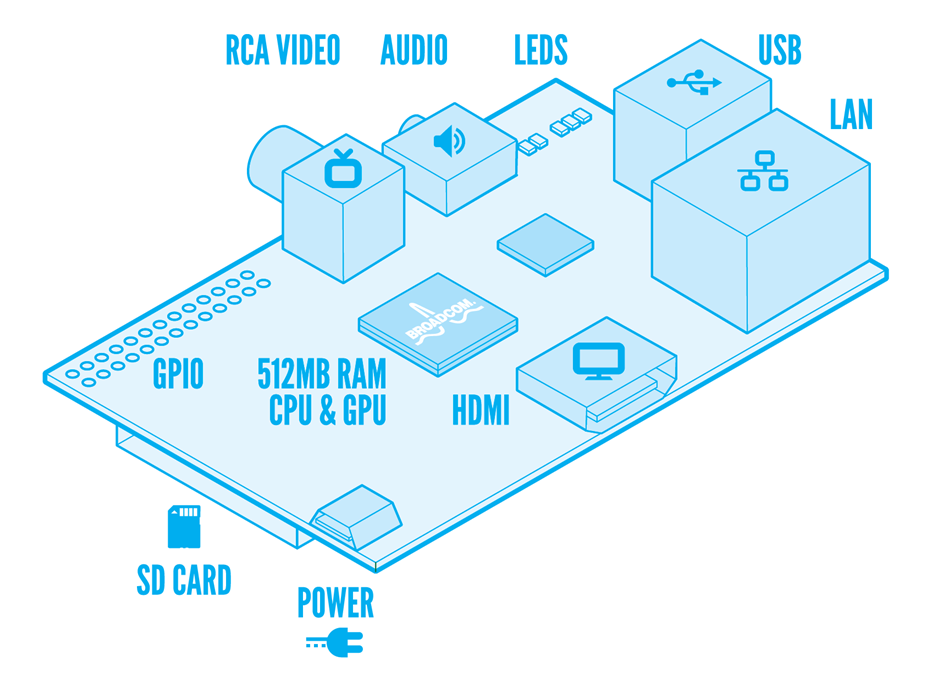
\includegraphics[width=0.8\textwidth]{Images/RaspberryPi.png}
        \caption{Diagram of the Raspberry Pi Model B}
        \label{fig:RaspberryPi}
    \end{figure}
\end{frame}

\subsection{Software}
\begin{frame}
    \frametitle{Server Software}
    \begin{itemize}
        \item {\large Raspian}
        \item {\large Apache2}
        \item {\large PostgreSQL}
    \end{itemize}
\end{frame}

\subsection{Chasis}
\begin{frame}
    \frametitle{Chasis Mock-up}
    \begin{figure}[htb]
        \centering
        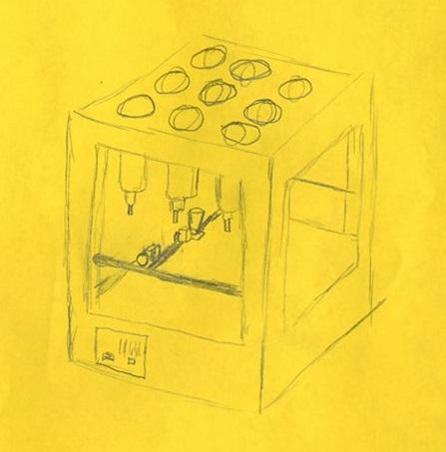
\includegraphics[width=0.6\textheight]{Images/ChasisMockup.png}
        \caption{Diagram of the Chasis}
        \label{fig:ChasisMockUp}
    \end{figure}
\end{frame}



\section{What We've Done}
\begin{frame}
    \frametitle{What We've Done}
    \begin{itemize}
        \item All teammates worked together on all documentation
        \item Hoang primarily worked on diagrams.
        \item Raspian installed
        \item Apache2, PostgreSQL installed
    \end{itemize}
\end{frame}


\section{Conclusion}
\begin{frame}
    \frametitle{Conclusion}
    {\large Why DRINC?}
\end{frame}


\end{document}
